% VISUAL-MANAGED-FILE
% Secondary empirical results retained for discussion and promotion when they
% sharpen our central economic interpretation.
% Generated by scripts/build_excess_use_date_fe_deck_values.py.
% Within-day cross-section of the excess-use construct: token-day intermediary
% count share on own endpoint count share, both in percentage points, date
% fixed effects absorbing the calendar. Provisional/E0 scope: the estimates run
% on the green route-only D3 panel and are not submission-authoritative until
% the findings freeze admits them. Refresh by rerunning
% scripts/run_excess_use_date_fe_ladder.py then this builder.
\newcommand{\DateFEPooledNative}{$+34.56$ pp}
\newcommand{\DateFEPooledNativeSE}{23.04 pp}
\newcommand{\DateFEPooledNativeCI}{$[-10.62, +79.75]$}
\newcommand{\DateFEPooledNativeP}{$p = 0.134$}
\newcommand{\DateFEPooledStable}{$+2.42$ pp}
\newcommand{\DateFEPooledStableSE}{1.32 pp}
\newcommand{\DateFEPooledStableCI}{$[-0.17, +5.01]$}
\newcommand{\DateFEPooledStableP}{$p = 0.067$}
\newcommand{\DateFEDayNative}{$+34.55$ pp}
\newcommand{\DateFEDayNativeSE}{23.04 pp}
\newcommand{\DateFEDayNativeCI}{$[-10.64, +79.74]$}
\newcommand{\DateFEDayNativeP}{$p = 0.134$}
\newcommand{\DateFEDayStable}{$+2.42$ pp}
\newcommand{\DateFEDayStableSE}{1.32 pp}
\newcommand{\DateFEDayStableCI}{$[-0.17, +5.01]$}
\newcommand{\DateFEDayStableP}{$p = 0.067$}
\newcommand{\DateFEDemandNative}{$+0.05$ pp}
\newcommand{\DateFEDemandNativeSE}{0.56 pp}
\newcommand{\DateFEDemandNativeCI}{$[-1.04, +1.14]$}
\newcommand{\DateFEDemandNativeP}{$p = 0.924$}
\newcommand{\DateFEDemandStable}{$+0.85$ pp}
\newcommand{\DateFEDemandStableSE}{0.50 pp}
\newcommand{\DateFEDemandStableCI}{$[-0.13, +1.83]$}
\newcommand{\DateFEDemandStableP}{$p = 0.090$}
\newcommand{\DateFEDemandImported}{$+0.14$ pp}
\newcommand{\DateFEDemandImportedSE}{0.11 pp}
\newcommand{\DateFEDemandImportedCI}{$[-0.08, +0.35]$}
\newcommand{\DateFEDemandImportedP}{$p = 0.207$}
\newcommand{\DateFEDemandStaked}{$+0.12$ pp}
\newcommand{\DateFEDemandStakedSE}{0.07 pp}
\newcommand{\DateFEDemandStakedCI}{$[-0.03, +0.26]$}
\newcommand{\DateFEDemandStakedP}{$p = 0.108$}
\newcommand{\DateFESlope}{1.587}
\newcommand{\DateFESlopeSE}{0.026}
\newcommand{\DateFESlopeCI}{$[+1.54, +1.64]$}
\newcommand{\DateFESlopeP}{$p < 0.001$}
\newcommand{\DateFESlopeWithinToken}{0.985}
\newcommand{\DateFESlopeWithinTokenSE}{0.301}
\newcommand{\DateFESlopeWithinTokenCI}{$[+0.39, +1.57]$}
\newcommand{\DateFESlopeWithinTokenP}{$p = 0.001$}
\newcommand{\DateFEStableMinusNative}{$+0.79$ pp}
\newcommand{\DateFEStableMinusNativeSE}{1.02 pp}
\newcommand{\DateFEStableMinusNativeCI}{$[-1.20, +2.78]$}
\newcommand{\DateFEStableMinusNativeP}{$p = 0.435$}
\newcommand{\DateFESlopeStableMinusNative}{0.351}
\newcommand{\DateFESlopeStableMinusNativeSE}{0.263}
\newcommand{\DateFESlopeStableMinusNativeCI}{$[-0.17, +0.87]$}
\newcommand{\DateFESlopeStableMinusNativeP}{$p = 0.183$}
\newcommand{\DateFESlopeNativeMinusImported}{0.075}
\newcommand{\DateFESlopeNativeMinusImportedSE}{0.028}
\newcommand{\DateFESlopeNativeMinusImportedCI}{$[+0.02, +0.13]$}
\newcommand{\DateFESlopeNativeMinusImportedP}{$p = 0.007$}
\newcommand{\DateFEWeightedNative}{$-15.91$ pp}
\newcommand{\DateFEWeightedNativeSE}{8.08 pp}
\newcommand{\DateFEWeightedNativeCI}{$[-31.76, -0.07]$}
\newcommand{\DateFEWeightedNativeP}{$p = 0.049$}
\newcommand{\DateFEWeightedSlope}{2.012}
\newcommand{\DateFEWeightedSlopeSE}{0.197}
\newcommand{\DateFEWeightedSlopeCI}{$[+1.63, +2.40]$}
\newcommand{\DateFEWeightedSlopeP}{$p < 0.001$}
\newcommand{\DateFECandidateNative}{$-17.45$ pp}
\newcommand{\DateFECandidateNativeSE}{7.63 pp}
\newcommand{\DateFECandidateNativeCI}{$[-32.41, -2.49]$}
\newcommand{\DateFECandidateNativeP}{$p = 0.022$}
\newcommand{\DateFECandidateImported}{$-1.34$ pp}
\newcommand{\DateFECandidateImportedSE}{0.62 pp}
\newcommand{\DateFECandidateImportedCI}{$[-2.55, -0.13]$}
\newcommand{\DateFECandidateImportedP}{$p = 0.030$}
\newcommand{\DateFEClassifiedNative}{$-1.51$ pp}
\newcommand{\DateFEClassifiedNativeSE}{1.27 pp}
\newcommand{\DateFEClassifiedNativeCI}{$[-4.09, +1.06]$}
\newcommand{\DateFEClassifiedNativeP}{$p = 0.240$}
\newcommand{\DateFEClassifiedImported}{$-0.64$ pp}
\newcommand{\DateFEClassifiedImportedSE}{0.48 pp}
\newcommand{\DateFEClassifiedImportedCI}{$[-1.62, +0.34]$}
\newcommand{\DateFEClassifiedImportedP}{$p = 0.192$}
\newcommand{\DateFEBackingOnChain}{$-0.77$ pp}
\newcommand{\DateFEBackingOnChainSE}{0.29 pp}
\newcommand{\DateFEBackingOnChainCI}{$[-1.35, -0.20]$}
\newcommand{\DateFEBackingOnChainP}{$p = 0.008$}
\newcommand{\DateFEBackingSynthetic}{$-0.61$ pp}
\newcommand{\DateFEBackingSyntheticSE}{0.26 pp}
\newcommand{\DateFEBackingSyntheticCI}{$[-1.11, -0.11]$}
\newcommand{\DateFEBackingSyntheticP}{$p = 0.017$}
\newcommand{\DateFEBackingRWA}{$-0.50$ pp}
\newcommand{\DateFEBackingRWASE}{0.33 pp}
\newcommand{\DateFEBackingRWACI}{$[-1.14, +0.14]$}
\newcommand{\DateFEBackingRWAP}{$p = 0.125$}
\newcommand{\DateFETether}{$-5.32$ pp}
\newcommand{\DateFETetherSE}{0.93 pp}
\newcommand{\DateFETetherCI}{$[-7.14, -3.51]$}
\newcommand{\DateFETetherP}{$p < 0.001$}
\newcommand{\DateFESlopeEarly}{1.605}
\newcommand{\DateFESlopeEarlySE}{0.034}
\newcommand{\DateFESlopeEarlyCI}{$[+1.54, +1.67]$}
\newcommand{\DateFESlopeEarlyP}{$p < 0.001$}
\newcommand{\DateFESlopeLate}{1.554}
\newcommand{\DateFESlopeLateSE}{0.026}
\newcommand{\DateFESlopeLateCI}{$[+1.50, +1.60]$}
\newcommand{\DateFESlopeLateP}{$p < 0.001$}
\newcommand{\DateFENativeEarly}{$+0.70$ pp}
\newcommand{\DateFENativeEarlySE}{0.98 pp}
\newcommand{\DateFENativeEarlyCI}{$[-1.22, +2.63]$}
\newcommand{\DateFENativeEarlyP}{$p = 0.473$}
\newcommand{\DateFENativeLate}{$-0.72$ pp}
\newcommand{\DateFENativeLateSE}{0.94 pp}
\newcommand{\DateFENativeLateCI}{$[-2.56, +1.12]$}
\newcommand{\DateFENativeLateP}{$p = 0.441$}
\newcommand{\DateFETokenDays}{1,828,862}
\newcommand{\DateFETokens}{304,572}
\newcommand{\DateFEDays}{2,259}
\newcommand{\DateFEAbsorbedDays}{2,259}
\newcommand{\DateFEWithinTokenAbsorbed}{306,830}
\newcommand{\DateFECandidateTokenDays}{11,233}
\newcommand{\DateFECandidateDays}{2,258}
\newcommand{\DateFEClassifiedTokenDays}{44,077}
\newcommand{\DateFEClassifiedTokens}{37}
\newcommand{\DateFECeilingMean}{0.0008}
\newcommand{\DateFECeilingNinetyNinth}{0.0004}
\newcommand{\DateFECeilingHalfShare}{0.08\%}
\newcommand{\DateFELeaveOutSlope}{3.209}
\newcommand{\DateFELeaveOutSlopeSE}{0.090}
\newcommand{\DateFEFloorFiveSlope}{1.579}
\newcommand{\DateFEFloorHundredSlope}{1.595}

% Generated by scripts/analyze/run_route_heterogeneity.py; do not edit.
% Supporting descriptive analysis; WETH eligibility is a mechanical sample boundary.
% SAMPLE: exact two-leg native-WETH-versus-stablecoin routes; 181 common month-days; 2024 versus January-June 2026
% LITERATURE-GROUNDING: Mukhin (2022) raw text lines 777-850 (trade-flow switching order); Gopinath-Stein (2021) lines 1280-1305 (share feedback); Carletti et al. (2021) lines 120-220 (funding-share substitution with unchanged total funding)
\newcommand{\WethCountFullChange}{$+21.1$ pp}
\newcommand{\WethCountFullCILower}{$+18.2$ pp}
\newcommand{\WethCountFullCIUpper}{$+24.0$ pp}
\newcommand{\WethCountNoEndpointChange}{$+3.7$ pp}
\newcommand{\WethCountNoEndpointCILower}{$+2.3$ pp}
\newcommand{\WethCountNoEndpointCIUpper}{$+5.2$ pp}
\newcommand{\WethCountWithinFullChange}{$+0.2$ pp}
\newcommand{\WethCountWithinFullCILower}{$-1.3$ pp}
\newcommand{\WethCountWithinFullCIUpper}{$+1.7$ pp}
\newcommand{\WethCountWithinNoEndpointChange}{$+0.3$ pp}
\newcommand{\WethCountWithinNoEndpointCILower}{$-1.9$ pp}
\newcommand{\WethCountWithinNoEndpointCIUpper}{$+2.6$ pp}
\newcommand{\WethValueFullChange}{$+27.2$ pp}
\newcommand{\WethValueFullCILower}{$+23.4$ pp}
\newcommand{\WethValueFullCIUpper}{$+30.9$ pp}
\newcommand{\WethValueNoEndpointChange}{$+21.5$ pp}
\newcommand{\WethValueNoEndpointCILower}{$+11.8$ pp}
\newcommand{\WethValueNoEndpointCIUpper}{$+31.1$ pp}
\newcommand{\WethValueActivityChange}{$+23.5$ pp}
\newcommand{\WethValueActivityCILower}{$+15.0$ pp}
\newcommand{\WethValueActivityCIUpper}{$+32.1$ pp}
\newcommand{\WethValueWithinChange}{$-2.0$ pp}
\newcommand{\WethValueWithinCILower}{$-9.8$ pp}
\newcommand{\WethValueWithinCIUpper}{$+5.7$ pp}
\newcommand{\WethCountMassBase}{26.6\%}
\newcommand{\WethCountMassEnd}{46.8\%}
\newcommand{\WethValueMassBase}{39.9\%}
\newcommand{\WethValueMassEnd}{60.5\%}
\newcommand{\WethCountMatchedGroups}{94,260}
\newcommand{\WethCountNoEndpointGroups}{79,347}

% Generated by scripts/tabulate/build_endpoint_direction_deck_values.py; do not edit.
% Exact common-calendar endpoint-direction contributions to the headline stable-share change.
\newcommand{\EndpointCountBase}{16.9\%}
\newcommand{\EndpointCountEnd}{42.3\%}
\newcommand{\EndpointCountChange}{$+25.4$ pp}
\newcommand{\EndpointCountChangeNumber}{25.4}
\newcommand{\EndpointOtherCountContribution}{$+15.2$ pp}
\newcommand{\EndpointOtherCountContributionNumber}{15.2}
\newcommand{\EndpointOtherCountShare}{59.8\%}
\newcommand{\EndpointNativeStableCountContribution}{$+9.2$ pp}
\newcommand{\EndpointNativeStableCountContributionNumber}{9.2}
\newcommand{\EndpointNativeStableCountShare}{36.2\%}
\newcommand{\EndpointStableStableCountContribution}{$+1.0$ pp}
\newcommand{\EndpointStableStableCountContributionNumber}{1.0}
\newcommand{\EndpointStableStableCountShare}{3.9\%}
\newcommand{\EndpointValueBase}{32.7\%}
\newcommand{\EndpointValueEnd}{76.5\%}
\newcommand{\EndpointValueChange}{$+43.9$ pp}
\newcommand{\EndpointValueChangeNumber}{43.9}
\newcommand{\EndpointOtherValueContribution}{$+20.6$ pp}
\newcommand{\EndpointOtherValueContributionNumber}{20.6}
\newcommand{\EndpointOtherValueShare}{46.8\%}
\newcommand{\EndpointNativeStableValueContribution}{$+10.1$ pp}
\newcommand{\EndpointNativeStableValueContributionNumber}{10.1}
\newcommand{\EndpointNativeStableValueShare}{23.0\%}
\newcommand{\EndpointStableStableValueContribution}{$+13.2$ pp}
\newcommand{\EndpointStableStableValueContributionNumber}{13.2}
\newcommand{\EndpointStableStableValueShare}{30.1\%}

% Generated by scripts/tabulate/build_stable_stable_vehicle_values.py; do not edit.
% Issuer identity within the stable-to-stable endpoint contribution.
\newcommand{\StableStableValueContribution}{$+13.2$ pp}
\newcommand{\StableStableUsdtValueContribution}{$+13.7$ pp}
\newcommand{\StableStableOtherValueContribution}{$-0.5$ pp}
\newcommand{\StableStableNativeValueContribution}{$+2.6$ pp}
\newcommand{\StableStableTrimmedValueChange}{$+12.3$ pp}
\newcommand{\StableStablePooledValueChange}{$+12.7$ pp}
\newcommand{\StableStableTrimmedBase}{5.0\%}
\newcommand{\StableStableTrimmedEnd}{17.3\%}
\newcommand{\StableStableActiveDays}{181}

% Generated by scripts/tabulate/render_network_position.py; do not edit.
\newcommand{\NetworkWethBetweennessTwentySix}{0.927}
\newcommand{\NetworkWethRankYears}{7}
\newcommand{\NetworkWethPositionTwentyFour}{76.2\%}
\newcommand{\NetworkWethPositionTwentySix}{42.3\%}
\newcommand{\NetworkStableDuoPositionTwentyFour}{14.9\%}
\newcommand{\NetworkStableDuoPositionTwentySix}{37.4\%}
\newcommand{\NetworkStableParticipationTwentyFour}{17.6\%}
\newcommand{\NetworkStableParticipationTwentySix}{46.1\%}

% Generated by scripts/tabulate/render_exact_vehicle_frontier.py; do not edit.
\newcommand{\ExactFrontierRoutes}{777{,}203}
\newcommand{\ExactFrontierDates}{73}
\newcommand{\ExactFrontierMinimumInput}{\$100}
\newcommand{\ExactFrontierGainThreshold}{1 bp}
\newcommand{\ExactFrontierImpactLimit}{5\%}
\newcommand{\ExactFrontierWithinShare}{6.6\%}
\newcommand{\ExactFrontierSameVehicleShare}{44.5\%}
\newcommand{\ExactFrontierAllPathShare}{46.4\%}
\newcommand{\ExactFrontierVehicleAddition}{2.0 pp}
\newcommand{\ExactFrontierMedianGain}{21.9 bp}
\newcommand{\ExactFrontierStableChange}{-1.2 pp}
\newcommand{\ExactFrontierStableDecline}{1.2 pp}
\newcommand{\ExactFrontierStableChangeSE}{0.2 pp}
\newcommand{\ExactFrontierStableValueChange}{-2.1 pp}
\newcommand{\ExactFrontierStableValueDecline}{2.1 pp}
\newcommand{\ExactFrontierHighNotionalChange}{-1.8 pp}
\newcommand{\ExactFrontierHighNotionalDecline}{1.8 pp}
\newcommand{\ExactFrontierHighNotionalRoutes}{78{,}627}
\newcommand{\ExactFrontierVenueCoverage}{93.4\%}
\newcommand{\ExactFrontierReproduction}{89.2\%}
\newcommand{\ExactFrontierExtremeRoutes}{98}

% Generated by scripts/tabulate/render_result_resolution_checks.py; do not edit.
\newcommand{\AdjacentLargestIncreaseYears}{2025--2026}
\newcommand{\AdjacentLargestIncrease}{$+17.4$ pp}
\newcommand{\AdjacentLargestDeclineYears}{2022--2023}
\newcommand{\AdjacentLargestDecline}{$-6.4$ pp}
\newcommand{\AdjacentWithinMin}{$-0.4$ pp}
\newcommand{\AdjacentWithinMax}{$+1.0$ pp}
\newcommand{\NonvehicleEndpointStableBase}{1.1\%}
\newcommand{\NonvehicleEndpointStableEnd}{9.0\%}
\newcommand{\NonvehicleEndpointStableChange}{$+8.0$ pp}
\newcommand{\NonvehicleEndpointCountExclusive}{$+7.2$ pp}
\newcommand{\NonvehicleEndpointValueBase}{0.9\%}
\newcommand{\NonvehicleEndpointValueEnd}{39.1\%}
\newcommand{\NonvehicleEndpointValueChange}{$+38.1$ pp}
\newcommand{\NonvehicleEndpointValueExclusive}{$+33.8$ pp}


% VISUAL-FUNCTION: graph position and realised use | three currency comparison columns | separate binary connectivity from intermediary allocation
\begin{frame}{A14. WETH stays the graph hub as realised use shifts}
\evidencekicker{All route lengths; monthly trading graphs}
\vspace{0.18cm}
\begin{columns}[T,totalwidth=0.92\textwidth]
\begin{column}{0.28\textwidth}
{\color{muted}\scriptsize WETH BETWENNESS\par}
{\fontsize{23}{25}\selectfont\bfseries\color{ucldark}\#1}\par
{\small in all \NetworkWethRankYears{} annual graphs\par}
\vspace{0.18cm}
{\large\bfseries\color{ucldark}\NetworkWethBetweennessTwentySix}\par
{\small in 2026 H1\par}
\end{column}
\hfill
\begin{column}{0.28\textwidth}
{\color{muted}\scriptsize WETH REALISED SHARE\par}
{\fontsize{22}{24}\selectfont\bfseries\color{ucldark}\NetworkWethPositionTwentyFour}\par
{\small 2024\par}
\vspace{0.16cm}
{\fontsize{22}{24}\selectfont\bfseries\color{accent}\NetworkWethPositionTwentySix}\par
{\small 2026 H1\par}
\end{column}
\hfill
\begin{column}{0.28\textwidth}
{\color{muted}\scriptsize USDC + USDT REALISED SHARE\par}
{\fontsize{22}{24}\selectfont\bfseries\color{muted}\NetworkStableDuoPositionTwentyFour}\par
{\small 2024\par}
\vspace{0.16cm}
{\fontsize{22}{24}\selectfont\bfseries\color{stable}\NetworkStableDuoPositionTwentySix}\par
{\small 2026 H1\par}
\end{column}
\end{columns}
\vspace{0.48cm}
{\large Binary network position changes much less than actual intermediary use.\par}
\decknote{Betweenness is approximate and unweighted in annual trading graphs built from trades on the fifteenth day of each month, using 256 source nodes and a fixed seed. Realised shares use all intermediary positions on the same dates. A graph edge records leg presence; realised routes add depth and execution cost.}
\end{frame}

% VISUAL-FUNCTION: endpoint demand and intermediary use | four-model regression table | show within-date demand pass-through and fixed-effect progression
\begin{frame}{A15. Endpoint demand predicts intermediary use}
\centering
{\scriptsize
\renewcommand{\arraystretch}{0.96}
\begin{tabularx}{0.94\textwidth}{@{}Xcccc@{}}
\toprule
 & \multicolumn{4}{c}{Intermediary share \((I_{a,t})\) [pp]} \\
\cmidrule(lr){2-5}
 & (1) & (2) & (3) & (4) \\
 & Pooled & Date FE & {}+ demand & {}+ currency FE \\
\midrule
Native currency & \DateFEPooledNativeTable{} & \DateFEDayNativeTable{} & \DateFEDemandNativeTable{} & --- \\
 & (\DateFEPooledNativeTableSE{}) & (\DateFEDayNativeTableSE{}) & (\DateFEDemandNativeTableSE{}) & --- \\
Stablecoin & \DateFEPooledStableTable{} & \DateFEDayStableTable{} & \DateFEDemandStableTable{} & --- \\
 & (\DateFEPooledStableTableSE{}) & (\DateFEDayStableTableSE{}) & (\DateFEDemandStableTableSE{}) & --- \\
Endpoint-demand share \((D_{a,t})\) & --- & --- & \DateFESlopeTable{} & \DateFESlopeWithinTokenTable{} \\
 & --- & --- & (\DateFESlopeTableSE{}) & (\DateFESlopeWithinTokenTableSE{}) \\
\midrule
Date fixed effects & No & Yes & Yes & Yes \\
Currency fixed effects & No & No & No & Yes \\
\bottomrule
\end{tabularx}\par}
\vspace{0.06cm}
{\footnotesize After date and currency effects, endpoint demand passes through almost one for one into intermediary use.\par}
\decknote{\DateFETokenDays{} currency-days over \DateFEDays{} dates. Parentheses report currency/date-clustered standard errors. The outcome and demand regressor are in pp. Currency effects absorb time-invariant asset-class indicators. Asterisks \(*\), \(**\), and \(***\) denote significance at 10\%, 5\%, and 1\%, respectively.}
\end{frame}

% VISUAL-FUNCTION: endpoint eligibility in the decomposition | two-branch composition diagram | isolate the mechanical WETH-endpoint component
% EVIDENCE-STATUS: supporting deterministic eligibility decomposition.
% EVIDENCE-SOURCES: output/exhibits/route_methodology_heterogeneity.jsonl; output/exhibits/route_methodology_heterogeneity_deck_values.tex
\begin{frame}{A16. Pair composition contains a mechanical component}
\vspace{-0.10cm}
\begin{center}
\resizebox{0.90\textwidth}{!}{% Presentation geometry only. Numerical labels are generated in
% output/exhibits/route_methodology_heterogeneity_deck_values.tex.
% WETH is the native intermediary in this comparison. If WETH is an endpoint,
% it cannot also be the intermediary; every such row therefore has stable_share=1.
\begin{tikzpicture}[x=1cm,y=1cm]
\tikzset{panel/.style={draw=rule,fill=white,rounded corners=3pt,line width=0.8pt}}
\tikzset{small/.style={font=\fontsize{6.8}{7.5}\selectfont,text=muted,align=center}}

\node[draw=stable,line width=1.1pt,circle,minimum size=1.05cm,
  font=\fontsize{8.2}{8.8}\selectfont\bfseries,text=ucldark] at (1.05,3.45) {WETH};
\node[anchor=west,font=\fontsize{8.2}{9.0}\selectfont\bfseries,text=ucldark]
  at (1.82,3.62) {WETH is an endpoint of the ultimate pair};
\node[anchor=west,font=\fontsize{7.2}{8.0}\selectfont,text=ink]
  at (1.82,3.25) {Stablecoins alone remain eligible as intermediaries.};

\draw[panel] (0,0.56) rectangle (6.00,2.68);
\node[anchor=west,font=\fontsize{8.1}{8.8}\selectfont\bfseries,text=ucldark]
  at (0.35,2.32) {All matched ultimate-pair groups};
\node[anchor=west,font=\fontsize{23}{24}\selectfont\bfseries,text=stable]
  at (0.35,1.48) {\WethCountFullChange};
\node[anchor=west,font=\fontsize{6.9}{7.6}\selectfont,text=muted]
  at (0.35,1.05) {95\% CI [\WethCountFullCILower, \WethCountFullCIUpper]};
\node[anchor=west,font=\fontsize{7.0}{7.7}\selectfont,text=ink]
  at (0.35,0.80) {WETH-linked route-count mass: \WethCountMassBase{} $\rightarrow$ \WethCountMassEnd};

\draw[panel] (6.35,0.56) rectangle (12.35,2.68);
\node[anchor=west,font=\fontsize{8.1}{8.8}\selectfont\bfseries,text=ucldark]
  at (6.70,2.32) {Ultimate-pair groups excluding WETH endpoints};
\node[anchor=west,font=\fontsize{23}{24}\selectfont\bfseries,text=accent]
  at (6.70,1.48) {\WethCountNoEndpointChange};
\node[anchor=west,font=\fontsize{6.9}{7.6}\selectfont,text=muted]
  at (6.70,1.05) {95\% CI [\WethCountNoEndpointCILower, \WethCountNoEndpointCIUpper]};
\node[anchor=west,font=\fontsize{7.0}{7.7}\selectfont,text=ink]
  at (6.70,0.80) {\WethCountNoEndpointGroups{} matched groups};

\node[small,text width=12.0cm] at (6.18,0.08)
  {\textbf{Within-ultimate-pair change:} all groups \WethCountWithinFullChange{} [\WethCountWithinFullCILower, \WethCountWithinFullCIUpper];\\excluding WETH endpoints \WethCountWithinNoEndpointChange{} [\WethCountWithinNoEndpointCILower, \WethCountWithinNoEndpointCIUpper].};
\end{tikzpicture}
}
\end{center}
\vspace{-0.08cm}
{\large Changes within fixed pairs are \WethCountWithinFullChange{} overall and \WethCountWithinNoEndpointChange{} after removing WETH endpoints.\par}
\decknote{A WETH endpoint mechanically excludes WETH as the intermediary. Exact two-leg native-WETH-versus-stablecoin routes on common month-days; fixed-pair estimates also absorb month-day and route scope.}
\end{frame}

% VISUAL-FUNCTION: endpoint direction and rotation | paired count-value contribution bars | distinguish broad count growth from stable-to-stable value concentration
\begin{frame}{A17. Endpoint direction splits count and value}
\vspace{-0.12cm}
\begin{center}
\resizebox{0.94\textwidth}{!}{% Presentation geometry only. Numerical labels are generated from
% output/exhibits/endpoint_direction_decomposition.jsonl.
\begin{tikzpicture}[x=1cm,y=1cm]
\tikzset{endpointpanel/.style={draw=rule,fill=white,rounded corners=3pt,line width=0.8pt}}
\tikzset{endpointlabel/.style={font=\fontsize{7.4}{8.2}\selectfont\bfseries,text=ucldark,align=left,text width=3.05cm}}
\path[use as bounding box] (0,0.05) rectangle (13.15,4.62);

\node[anchor=west,font=\fontsize{8.2}{9.0}\selectfont\bfseries,text=muted] at (0.10,4.37) {CONTRIBUTION TO THE STABLECOIN-SHARE INCREASE};

\draw[endpointpanel] (0.05,0.22) rectangle (6.40,4.08);
\node[anchor=west,font=\fontsize{15}{16}\selectfont\bfseries,text=stable] at (0.35,3.61) {Route count: \EndpointCountChange};
\node[endpointlabel,anchor=west] at (0.35,2.81) {Other endpoint pairs};
\fill[stable!85] (3.35,2.58) rectangle ({3.35+0.12*\EndpointOtherCountContributionNumber},2.99);
\node[anchor=west,font=\fontsize{8.3}{9}\selectfont\bfseries,text=ink] at (5.28,2.78) {\EndpointOtherCountContribution};
\node[endpointlabel,anchor=west] at (0.35,1.91) {One native, one stable};
\fill[accent!85] (3.35,1.68) rectangle ({3.35+0.12*\EndpointNativeStableCountContributionNumber},2.09);
\node[anchor=west,font=\fontsize{8.3}{9}\selectfont\bfseries,text=ink] at (4.57,1.88) {\EndpointNativeStableCountContribution};
\node[endpointlabel,anchor=west] at (0.35,1.01) {Two stable endpoints};
\fill[ucldark!75] (3.35,0.78) rectangle ({3.35+0.12*\EndpointStableStableCountContributionNumber},1.19);
\node[anchor=west,font=\fontsize{8.3}{9}\selectfont\bfseries,text=ink] at (3.62,0.98) {\EndpointStableStableCountContribution};

\draw[endpointpanel] (6.70,0.22) rectangle (13.10,4.08);
\node[anchor=west,font=\fontsize{15}{16}\selectfont\bfseries,text=stable] at (7.00,3.61) {Routed value: \EndpointValueChange};
\node[endpointlabel,anchor=west] at (7.00,2.81) {Other endpoint pairs};
\fill[stable!85] (10.00,2.58) rectangle ({10.00+0.10*\EndpointOtherValueContributionNumber},2.99);
\node[anchor=west,font=\fontsize{8.3}{9}\selectfont\bfseries,text=ink] at (12.16,2.78) {\EndpointOtherValueContribution};
\node[endpointlabel,anchor=west] at (7.00,1.91) {One native, one stable};
\fill[accent!85] (10.00,1.68) rectangle ({10.00+0.10*\EndpointNativeStableValueContributionNumber},2.09);
\node[anchor=west,font=\fontsize{8.3}{9}\selectfont\bfseries,text=ink] at (11.16,1.88) {\EndpointNativeStableValueContribution};
\node[endpointlabel,anchor=west] at (7.00,1.01) {Two stable endpoints};
\fill[ucldark!75] (10.00,0.78) rectangle ({10.00+0.10*\EndpointStableStableValueContributionNumber},1.19);
\node[anchor=west,font=\fontsize{8.3}{9}\selectfont\bfseries,text=ink] at (11.42,0.98) {\EndpointStableStableValueContribution};
\end{tikzpicture}
}
\end{center}
\vspace{-0.08cm}
{\large USDT supplies \StableStableUsdtValueContribution{} of the \StableStableValueContribution{} two-stable-endpoint value channel.\par}
\decknote{Exact additive decomposition on 181 matched dates in 2024 and 2026. Endpoint direction describes the pair; the vehicle remains the intermediary token.}
\end{frame}

% VISUAL-FUNCTION: window and endpoint restrictions | three compact estimates | show that composition explains reversals and survives nonvehicle endpoints
% EVIDENCE-STATUS: direct robustness decompositions.
% EVIDENCE-SOURCES: output/exhibits/vehicle_transition_adjacent_year_decomposition.jsonl; output/exhibits/vehicle_transition_nonvehicle_endpoint_decomposition.jsonl; output/exhibits/result_resolution_values.tex
\begin{frame}{A17b. Rotation survives time and endpoint restrictions}
\vspace{0.18cm}
\begin{columns}[T,totalwidth=0.92\textwidth]
\begin{column}{0.29\textwidth}
\centering
{\fontsize{18}{20}\selectfont\bfseries\color{ucldark}\AdjacentWithinMin{} to\\[-0.03cm] \AdjacentWithinMax}\par
{\small within-pair term across\\all adjacent H1 comparisons\par}
\end{column}
\hfill
\begin{column}{0.29\textwidth}
\centering
{\fontsize{19}{21}\selectfont\bfseries\color{stable}\NonvehicleEndpointStableBase{} $\rightarrow$\\[-0.03cm] \NonvehicleEndpointStableEnd}\par
{\small route-count share with\\nonvehicle endpoints\par}
\end{column}
\hfill
\begin{column}{0.29\textwidth}
\centering
{\fontsize{19}{21}\selectfont\bfseries\color{stable}\NonvehicleEndpointValueBase{} $\rightarrow$\\[-0.03cm] \NonvehicleEndpointValueEnd}\par
{\small supported-value share with\\nonvehicle endpoints\par}
\end{column}
\end{columns}
\vspace{0.62cm}
{\large Pair entry and exit contribute \NonvehicleEndpointCountExclusive{} by count and \NonvehicleEndpointValueExclusive{} by value.\par}
\decknote{Adjacent comparisons use matched January--June dates from 2019 through 2026. The endpoint restriction removes every pair with WETH or a stablecoin at either endpoint. All changes and components are in pp; supported value applies the 20\% agreement rule.}
\end{frame}

% VISUAL-FUNCTION: local and network liquidity | three coefficient columns | compare bridge depth with broader network reach
\begin{frame}{A18. Local depth remains informative alongside network reach}
\vspace{0.18cm}
\begin{columns}[T,totalwidth=0.92\textwidth]
\begin{column}{0.28\textwidth}
{\fontsize{24}{26}\selectfont\bfseries\color{ucldark}\BridgeLiquidityTopShare}\par
{\small of routes use the deepest supported bridge\par}
\end{column}
\hfill
\begin{column}{0.28\textwidth}
{\fontsize{24}{26}\selectfont\bfseries\color{stable}\BridgeLiquidityHorseRaceDepthCoef}\par
{\small route share per log point of weak-leg capital\par}
\end{column}
\hfill
\begin{column}{0.28\textwidth}
{\fontsize{24}{26}\selectfont\bfseries\color{uclbright}\BridgeLiquidityHorseRaceGlobalDayCoef}\par
{\small route share per log point of same-day network reach\par}
\end{column}
\end{columns}
\vspace{0.68cm}
{\large Local two-leg depth and broader network position both matter.\par}
\decknote{Five vehicle currencies compared within the same set defined by pair, date, and route scope. Depth is prior-calendar deposited capital on the weaker leg. The regression absorbs set and vehicle effects and clusters by pair and date.}
\end{frame}

% VISUAL-FUNCTION: source of pre-use capital | three capital-allocation estimates | distinguish deepening from newly active pools
\begin{frame}{A19. First-use capital lies in active pools}
\evidencekicker{Supported stablecoin, day -7 to first use}
\vspace{0.20cm}
\begin{columns}[T,totalwidth=0.92\textwidth]
\begin{column}{0.28\textwidth}
{\fontsize{24}{26}\selectfont\bfseries\color{stable}\BridgePoolMarginContinuingCapitalShare}\par
{\small of first-use capital lies in continuing pools\par}
\end{column}
\hfill
\begin{column}{0.28\textwidth}
{\fontsize{24}{26}\selectfont\bfseries\color{ucldark}\BridgePoolMarginContinuingDifference}\par
{\small continuing-pool growth relative to WETH\par}
\end{column}
\hfill
\begin{column}{0.28\textwidth}
{\fontsize{24}{26}\selectfont\bfseries\color{stable}\BridgePoolMarginNewPoolDifference}\par
{\small greater probability of a newly active pool\par}
\end{column}
\end{columns}
\decknote{\BridgePoolMarginEvents{} first-use events. A newly active pool has positive prior-calendar capital on day zero and none on day -7; continuing pools are positive on both dates. Difference inference clusters by pair and adoption date.}
\end{frame}

% EVIDENCE-STATUS: descriptive depth association supporting the contestable route-choice result.
% EVIDENCE-SOURCES: output/exhibits/bridge_liquidity_dominance.jsonl.
% VISUAL-FUNCTION: relative depth and route use | ordered depth blocks | show how a supported bridge becomes competitive
\begin{frame}{A20. Relative depth predicts route flow}
\evidencekicker{First 30 days after persistent stablecoin support}
\vspace{0.05cm}
\begin{center}
\begin{tikzpicture}[x=1cm,y=1cm]
\node[softbox,text width=3.25cm,minimum height=1.70cm,align=center] (thin) at (-4.25,1.35)
{\small Below $0.1\times$ WETH depth\\[0.14cm]{\fontsize{24}{26}\selectfont\bfseries\color{muted}\BridgeDepthThinFirstShare}};
\node[softbox,text width=3.25cm,minimum height=1.70cm,align=center,fill=stable!7] (equal) at (0,1.35)
{\small At least WETH depth\\[0.14cm]{\fontsize{24}{26}\selectfont\bfseries\color{stable}\BridgeDepthEqualFirstShare}};
\node[softbox,text width=3.25cm,minimum height=1.70cm,align=center,fill=stable!12] (double) at (4.25,1.35)
{\small At least $2\times$ WETH depth\\[0.14cm]{\fontsize{24}{26}\selectfont\bfseries\color{stable}\BridgeDepthDoubleFirstShare}};
\draw[-{Stealth[length=7pt]},line width=1.6pt,draw=stable] (thin)--(equal);
\draw[-{Stealth[length=7pt]},line width=1.6pt,draw=stable] (equal)--(double);
\end{tikzpicture}
\end{center}
\vspace{0.28cm}
{\large\bfseries Vehicle competition turns on relative depth.\par}
\decknote{Depth is prior-calendar deposited capital on the weaker leg. The route-share comparison uses \BridgeDepthDoseFirstRows{} pair-days across \BridgeDepthDoseFirstEvents{} bridge events. Support and depth refer to the same stablecoin set. Capital and route demand are jointly determined.}
\end{frame}

% EVIDENCE-STATUS: descriptive first-use comparison with economic interpretations of liquidity supply.
% EVIDENCE-SOURCES: output/exhibits/bridge_liquidity_dominance.jsonl; Milionis et al. (2022).
% VISUAL-FUNCTION: support to first use | two probability blocks | separate binary support from usable depth
\begin{frame}{A21. Usable depth turns support into first use}
\evidencekicker{Probability of first stablecoin use within 30 days}
\vspace{0.34cm}
\begin{columns}[T,totalwidth=0.86\textwidth]
\begin{column}{0.38\textwidth}
\begin{beamercolorbox}[rounded=true,sep=0.40cm,wd=\textwidth]{block body}
{\small\color{muted} BELOW $0.1\times$ WETH DEPTH\par}\vspace{0.12cm}
{\fontsize{30}{32}\selectfont\bfseries\color{accent}\BridgeTimingShallowMonthShare\par}
\end{beamercolorbox}
\end{column}
\begin{column}{0.10\textwidth}\centering\vspace{0.70cm}{\Large$\rightarrow$}\end{column}
\begin{column}{0.38\textwidth}
\begin{beamercolorbox}[rounded=true,sep=0.40cm,wd=\textwidth]{block body}
{\small\color{muted} AT LEAST $0.1\times$ WETH DEPTH\par}\vspace{0.12cm}
{\fontsize{30}{32}\selectfont\bfseries\color{stable}\BridgeTimingCompetitiveMonthShare\par}
\end{beamercolorbox}
\end{column}
\end{columns}
\vspace{0.48cm}
{\large Positive pool capital becomes useful as both route legs deepen.\par}
\decknote{The sample follows \BridgeTimingEvents{} pair events after persistent support appears. The estimates compare first use within 30 days. Lower divergence loss and issuer-linked pool seeding are two possible supply channels. Provider profitability also depends on entry prices, fee income, hedges, and expectations.}
\end{frame}

% EVIDENCE-STATUS: descriptive event-time capital path among eventual users.
% EVIDENCE-SOURCES: output/figures/experiments/bridge_adoption_capital_path.pdf; output/exhibits/bridge_liquidity_dominance.jsonl.
% VISUAL-FUNCTION: capital before first use | event-time line chart and two estimates | show depth building into observed routing
\begin{frame}{A22. Bridge capital builds before first use}
\evidencekicker{Supported stablecoin first used at day zero}
\vspace{0.02cm}
\begin{columns}[T,totalwidth=0.95\textwidth]
\begin{column}{0.66\textwidth}
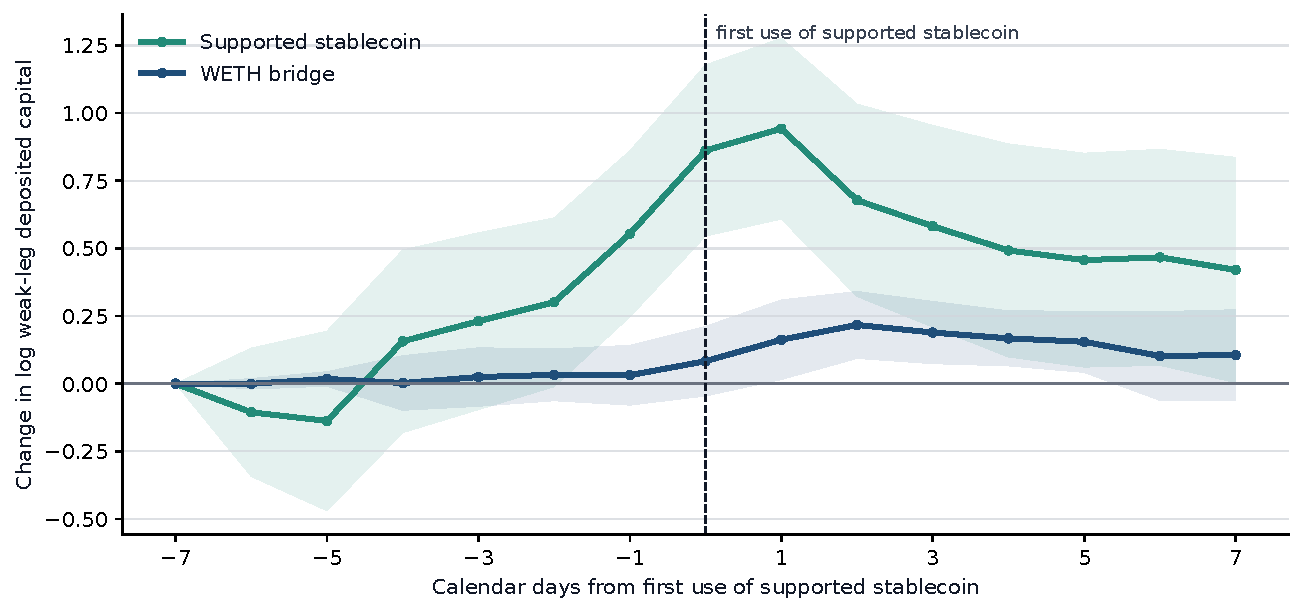
\includegraphics[width=\textwidth,height=0.65\textheight,keepaspectratio]{../output/figures/experiments/bridge_adoption_capital_path.pdf}
\end{column}
\hfill
\begin{column}{0.27\textwidth}
{\color{muted}\scriptsize BEFORE FIRST USE\par}\vspace{0.05cm}
{\fontsize{23}{25}\selectfont\bfseries\color{stable}\BridgeAdoptionCapitalPreCoef\par}
{\small stablecoin bridge, day -7 to 0\par}
\vspace{0.38cm}
{\color{muted}\scriptsize AFTER FIRST USE\par}\vspace{0.05cm}
{\fontsize{23}{25}\selectfont\bfseries\color{accent}\BridgeAdoptionCapitalPostCoef\par}
{\small stablecoin bridge, day 0 to +7\par}
\end{column}
\end{columns}
\vspace{0.02cm}
{\large Capital builds into first use, then partly unwinds.\par}
\decknote{\BridgeAdoptionCapitalEvents{} pair events with first use 7 to 119 days after persistent support. Relative to WETH, capital changes \BridgeAdoptionCapitalMatchedPreCoef{} before and \BridgeAdoptionCapitalMatchedPostCoef{} after first use. \BridgePoolMarginContinuingCapitalShare{} of first-use capital lies in pools active one week earlier. Capital is lagged one day; intervals cluster by pair and adoption date.}
\end{frame}

% EVIDENCE-STATUS: exact pre-transaction opportunity-set comparison.
% EVIDENCE-SOURCES: output/exhibits/exact_vehicle_frontier_monthly.jsonl.
% VISUAL-FUNCTION: venue and vehicle price competition | nested opportunity-set blocks | separate venue improvement from vehicle replacement
\begin{frame}{A23. Broader price search mostly changes the venue}
\evidencekicker{Share of routes with a quote more than 1 bp better than execution}
\vspace{0.08cm}
\begin{columns}[T,totalwidth=0.94\textwidth]
\begin{column}{0.26\textwidth}
\begin{beamercolorbox}[rounded=true,sep=0.30cm,wd=\textwidth]{block body}
{\color{muted}\scriptsize SAME VEHICLE, USED VENUES\par}\vspace{0.10cm}
{\fontsize{25}{27}\selectfont\bfseries\color{ucldark}\ExactFrontierWithinShare\par}
\end{beamercolorbox}
\end{column}
\begin{column}{0.05\textwidth}\centering\vspace{0.56cm}{\large$\rightarrow$}\end{column}
\begin{column}{0.26\textwidth}
\begin{beamercolorbox}[rounded=true,sep=0.30cm,wd=\textwidth]{block body}
{\color{muted}\scriptsize SAME VEHICLE, ALL EXACT VENUES\par}\vspace{0.10cm}
{\fontsize{25}{27}\selectfont\bfseries\color{stable}\ExactFrontierSameVehicleShare\par}
\end{beamercolorbox}
\end{column}
\begin{column}{0.05\textwidth}\centering\vspace{0.56cm}{\large$\rightarrow$}\end{column}
\begin{column}{0.26\textwidth}
\begin{beamercolorbox}[rounded=true,sep=0.30cm,wd=\textwidth]{block body}
{\color{muted}\scriptsize ANY VEHICLE OR DIRECT\par}\vspace{0.10cm}
{\fontsize{25}{27}\selectfont\bfseries\color{stable}\ExactFrontierAllPathShare\par}
\end{beamercolorbox}
\end{column}
\end{columns}
\vspace{0.44cm}
{\large Opening other vehicles adds \ExactFrontierVehicleAddition{}; stablecoin share changes by \ExactFrontierStableChange{}.\par}
\decknote{Routes are repriced for the same pair and input immediately before execution. The sample contains \ExactFrontierRoutes{} routes on \ExactFrontierDates{} monthly dates across exact Uniswap v2, SushiSwap v2, and Uniswap v3 states; minimum input is \ExactFrontierMinimumInput{} and the impact limit is \ExactFrontierImpactLimit{}. Quotes are gross of gas.}
\end{frame}

% EVIDENCE-STATUS: robustness of corrected persistence to stronger entry-day support.
% EVIDENCE-SOURCES: output/exhibits/entry_vehicle_persistence_models.jsonl; output/exhibits/entry_vehicle_persistence_support.jsonl.
% VISUAL-FUNCTION: persistence robustness | two support rows and two horizons | show stability when entry vehicle use is measured more precisely
\begin{frame}{A24. Persistence is equally strong on busy entry days}
\evidencekicker{Effect of 10 pp more stablecoin use on the entry day}
\vspace{0.18cm}
\begin{center}
\renewcommand{\arraystretch}{1.45}
\begin{tabularx}{0.86\textwidth}{@{}>{\raggedright\arraybackslash}Xcc@{}}
\toprule
 & Days 1--30 & Days 31--120 \\
\midrule
At least 5 entry routes & \textbf{\color{ucldark}\EntryPersistenceEarlyMinFiveEffectPerTen} & \textbf{\color{ucldark}\EntryPersistenceLateMinFiveEffectPerTen} \\
At least 10 entry routes & \textbf{\color{stable}\EntryPersistenceEarlyMinTenEffectPerTen} & \textbf{\color{stable}\EntryPersistenceLateMinTenEffectPerTen} \\
\bottomrule
\end{tabularx}
\end{center}
\vspace{0.48cm}
{\large\bfseries\color{ucldark}\centering Stronger entry measurement leaves the persistence estimate intact.\par}
\decknote{The entry day is excluded and the follow-up windows are disjoint. The 5-route samples contain \EntryPersistenceEarlyMinFivePairs{} and \EntryPersistenceLateMinFivePairs{} pairs; the 10-route samples contain \EntryPersistenceEarlyMinTenPairs{} and \EntryPersistenceLateMinTenPairs{}. Controls match the main pair-weighted specification, and standard errors cluster by entry date.}
\end{frame}

% EVIDENCE-STATUS: boundary test relating prior relative-price risk to constant-product bridge capital.
% EVIDENCE-SOURCES: output/exhibits/bridge_lp_divergence_risk_models.jsonl; output/exhibits/bridge_lp_divergence_risk_support.jsonl; output/tables/bridge_lp_divergence_risk.tex.
% VISUAL-FUNCTION: divergence risk and bridge capital | directional regression and cross-family comparison | delimit the liquidity-supply interpretation
\begin{frame}{A25. Divergence risk helps locate bridge capital}
\evidencekicker{Effect of 10 pp more prior relative volatility}
\vspace{0.20cm}
\begin{columns}[T,totalwidth=0.90\textwidth]
\begin{column}{0.41\textwidth}
\begin{beamercolorbox}[rounded=true,sep=0.32cm,wd=\textwidth]{block body}
{\small\color{muted} LOG BRIDGE CAPITAL\par}
\vspace{0.14cm}
{\fontsize{23}{25}\selectfont\bfseries\color{ucldark}\BridgeRiskCurrentVolEffect\par}
{\small current date\quad (\BridgeRiskCurrentVolSE)\par}
\vspace{0.18cm}
{\fontsize{23}{25}\selectfont\bfseries\color{stable}\BridgeRiskFutureVolEffect\par}
{\small 30 days later\quad (\BridgeRiskFutureVolSE)\par}
\end{beamercolorbox}
\end{column}
\hfill
\begin{column}{0.41\textwidth}
\begin{beamercolorbox}[rounded=true,sep=0.32cm,wd=\textwidth]{block body}
{\small\color{muted} MEDIAN RELATIVE VOLATILITY\par}
\vspace{0.14cm}
{\large\bfseries\color{ucldark}Native\quad \BridgeRiskNativeMedianVol\par}
\vspace{0.18cm}
{\large\bfseries\color{accent}Stablecoin\quad \BridgeRiskStableMedianVol\par}
\vspace{0.18cm}
{\small Stablecoin bridge has lower risk in \textbf{\BridgeRiskStableLowerShare} of pair-months.}
\end{beamercolorbox}
\end{column}
\end{columns}
\vspace{0.36cm}
{\large\bfseries\color{stable}\centering Risk shapes local capital; the rotation extends beyond it.\par}
\decknote{The panel contains \BridgeRiskObservations{} constant-product WETH and stablecoin bridge observations with positive capital on both legs. Models absorb pair-by-date and vehicle effects, control for prior route activity, and cluster by \BridgeRiskPairClusters{} pairs and \BridgeRiskDateClusters{} dates. Daily divergence loss gives the same directional result. The outcome is deposited capital; provider returns remain outside measurement.}
\end{frame}
